\chapter[Anhang]{Anhang}

\section{Erhobene GitHub Daten}

Die erhobenen GitHub Daten werden aufgeteilt auf 6 Seiten. Teil 1 bis Teil 3. Wobei jeder Teil nochmal in 2 subparts unterteilt ist,
da die Tabellen mit allen Attributen sehr breit sind. Die \textit{Parts} ergänzen die Tabelle um Spalten, die \textit{Teile} ergänzen die Tabelle, um Zeilen.

Würde man die Tabellen nebeneinander legen wäre sie wie folgt zu lesen:

\begin{table}[h]
    \begin{tabular}{|l|l|}
        \hline
        Teil 1, Part 1 & Teil 1, Part 2 \\ \hline
        Teil 2, Part 1 & Teil 1, Part 2 \\ \hline
        Teil 3, Part 1 & Teil 3, Part 3 \\ \hline
    \end{tabular}%
\end{table}

% ---------------------------------------- Teil 1, Part 1 ---------------------------------------- %
\begin{landscape}
    \begin{table}[h]
        \resizebox{\textwidth}{!}{%
            \begin{tabular}{lllccclll}
                   & \textbf{GitHub\_Project}  & \textbf{NPM\_package} & \textbf{Documentation} & \textbf{Sponsors} & \textbf{BackedBy} & \textbf{Category} & \textbf{created\_at} & \textbf{stars} \\ \hline
                0  & axios/axios               & axios                 & 2                      & 1                 & 0                 & Library           & 2014-08-18T22:30:27Z & 93419          \\ \hline
                1  & mrdoob/three.js           & three                 & 2                      & 1                 & 0                 & UI                & 2010-03-23T18:58:01Z & 82050          \\ \hline
                2  & angular/angular           & @angular/core         & 2                      & 0                 & 2                 & Framework         & 2014-09-18T16:12:01Z & 81406          \\ \hline
                3  & mui/material-ui           & @mui/material         & 2                      & 1                 & 0                 & UI                & 2014-08-18T19:11:54Z & 78499          \\ \hline
                4  & storybookjs/storybook     & @storybook/core       & 2                      & 1                 & 0                 & Utility           & 2016-03-18T04:23:44Z & 71018          \\ \hline
                5  & atom/atom                 &                       & 1                      & 0                 & 2                 & Application       & 2012-01-20T18:18:21Z & 57548          \\ \hline
                6  & expressjs/express         & express               & 1                      & 0                 & 1                 & Framework         & 2009-06-26T18:56:01Z & 57033          \\ \hline
                7  & chartjs/Chart.js          & chart.js              & 2                      & 0                 & 0                 & UI                & 2013-03-17T23:56:36Z & 56951          \\ \hline
                8  & lodash/lodash             & lodash                & 2                      & 0                 & 1                 & Library           & 2012-04-07T04:11:46Z & 53221          \\ \hline
                9  & jashkenas/underscore      & underscore            & 1                      & 1                 & 0                 & Library           & 2009-10-25T18:31:06Z & 26424          \\ \hline
                10 & ElemeFE/element           & element-ui            & 2                      & 1                 & 0                 & UI                & 2016-09-03T06:19:26Z & 52095          \\ \hline
                11 & elemefe/element-react     & element-react         & 2                      & 0                 & 0                 & UI                & 2016-10-18T06:56:20Z & 2718           \\ \hline
                12 & element-plus/element-plus & element-plus          & 2                      & 1                 & 0                 & UI                & 2020-07-21T06:51:19Z & 15561          \\ \hline
                13 & facebook/react            & react                 & 2                      & 0                 & 2                 & Library           & 2013-05-24T16:15:54Z & 188137         \\ \hline
                14 & chalk/chalk               & chalk                 & 1                      & 1                 & 0                 & UI                & 2013-08-03T00:20:12Z & 18514          \\ \hline
                15 & reduxjs/redux             & redux                 & 1                      & 1                 & 0                 & Library           & 2015-05-29T23:53:15Z & 58052          \\ \hline
                16 & vitejs/vite               & vite                  & 2                      & 1                 & 0                 & Utility           & 2020-04-21T05:03:57Z & 41817          \\ \hline
                17 & meteor/meteor             & meteor                & 2                      & 0                 & 2                 & Framework         & 2012-01-19T01:58:17Z & 42888          \\ \hline
                18 & nestjs/nest               & @nestjs/core          & 2                      & 1                 & 0                 & Framework         & 2017-02-04T20:12:52Z & 47005          \\ \hline
                19 & mermaid-js/mermaid        &                       & 2                      & 1                 & 0                 & Application       & 2014-11-01T23:52:32Z & 47280          \\ \hline
                20 & serverless/serverless     & serverless            & 1                      & 0                 & 2                 & Framework         & 2015-04-21T03:48:40Z & 42759          \\ \hline
                21 & juliangarnier/anime       & animejs               & 2                      & 0                 & 0                 & UI                & 2016-03-13T21:37:45Z & 42291          \\ \hline
                22 & microsoft/vscode          &                       & 1                      & 0                 & 2                 & Open-Core         & 2015-09-03T20:23:38Z & 131809         \\ \hline
                23 & vercel/next.js            & next                  & 1                      & 0                 & 2                 & Framework         & 2016-10-05T23:32:51Z & 86860          \\ \hline
                24 & coder/code-server         &                       & 1                      & 0                 & 2                 & Application       & 2019-02-27T16:50:41Z & 53554          \\ \hline
                25 & apache/echarts            & echarts               & 2                      & 0                 & 1                 & UI                & 2013-04-03T03:18:59Z & 51078          \\ \hline
                26 & sequelize/sequelize       & sequelize             & 1                      & 1                 & 0                 & ORM               & 2010-07-22T07:11:11Z & 26145          \\ \hline
                27 & wwayne/react-tooltip      & react-tooltip         & 2                      & 0                 & 0                 & UI                & 2015-04-07T13:15:04Z & 2752           \\ \hline
                28 & d3/d3                     & d3                    & 2                      & 0                 & 0                 & UI                & 2010-09-27T17:22:42Z & 101304         \\ \hline
                29 & recharts/recharts         & recharts              & 2                      & 1                 & 0                 & UI                & 2015-08-07T06:50:27Z & 18239          \\ \hline
                30 & plotly/plotly.js          & plotly.js             & 2                      & 1                 & 2                 & UI                & 2015-11-05T23:27:17Z & 14668          \\ \hline
                31 & typeorm/typeorm           & typeorm               & 1                      & 1                 & 0                 & ORM               & 2016-02-29T07:41:14Z & 28251          \\ \hline
                32 & moment/moment             & moment                & 1                      & 0                 & 1                 & Library           & 2011-03-01T02:46:06Z & 46534          \\ \hline
                33 & fastify/fastify           & fastify               & 1                      & 1                 & 1                 & Framework         & 2016-09-28T19:10:14Z & 23098          \\ \hline
                34 & Unitech/pm2               & pm2                   & 1                      & 0                 & 2                 & Utility           & 2013-05-21T03:25:25Z & 37005          \\ \hline
                35 & moment/luxon              & luxon                 & 1                      & 0                 & 1                 & Library           & 2015-11-30T12:48:48Z & 12466
            \end{tabular}%
        }
        \caption*{Teil 1, Part 1}
    \end{table}
\end{landscape}





% ---------------------------------------- Teil 1, Part 2 ---------------------------------------- %

\begin{landscape}
    \begin{table}[h]
        \resizebox{\textwidth}{!}{%
            \begin{tabular}{lcclllllll}
                   & \textbf{code\_of\_conduct} & \textbf{contributing} & \textbf{license} & \textbf{commits} & \textbf{contributors} & \textbf{last12MonthsCommits} & \textbf{usedBy} & \textbf{downloads} & \textbf{dependants} \\ \hline
                0  & 1                          & 1                     & mit              & 1199             & 367                   & 151                          & 6333706.0       & 30140843           & 77979               \\ \hline
                1  & 1                          & 1                     & mit              & 40103            & 1625                  & 1685                         & 0.0             & 628367             & 2359                \\ \hline
                2  & 1                          & 1                     & mit              & 24510            & 1547                  & 2500                         & 1913102.0       & 3163072            & 12467               \\ \hline
                3  & 1                          & 1                     & mit              & 19695            & 2513                  & 2596                         & 867211.0        & 1271064            & 1478                \\ \hline
                4  & 1                          & 1                     & mit              & 39819            & 1494                  & 0                            & 3438.0          & 3973351            & 108                 \\ \hline
                5  & 1                          & 1                     & mit              & 38496            & 489                   & 151                          & 0.0             & 0                  & 68                  \\ \hline
                6  & 1                          & 1                     & mit              & 5734             & 293                   & 110                          & 0.0             & 25466973           & 61798               \\ \hline
                7  & 0                          & 1                     & mit              & 4190             & 411                   & 266                          & 519078.0        & 2088541            & 2335                \\ \hline
                8  & 1                          & 1                     & mit              & 8005             & 310                   & 0                            & 15508835.0      & 44787010           & 155392              \\ \hline
                9  & 1                          & 1                     & mit              & 2797             & 280                   & 38                           & 1491035.0       & 9144831            & 22303               \\ \hline
                10 & 0                          & 1                     & mit              & 4532             & 569                   & 83                           & 268187.0        & 311656             & 8664                \\ \hline
                11 & 0                          & 1                     & mit              & 1236             & 48                    & 0                            & 2233.0          & 2560               & 33                  \\ \hline
                12 & 1                          & 1                     & mit              & 3462             & 313                   & 2352                         & 19233.0         & 81650              & 744                 \\ \hline
                13 & 1                          & 1                     & mit              & 14979            & 1557                  & 795                          & 10052259.0      & 15117154           & 86909               \\ \hline
                14 & 1                          & 1                     & mit              & 332              & 53                    & 15                           & 15166164.0      & 175939084          & 0                   \\ \hline
                15 & 1                          & 1                     & mit              & 3530             & 907                   & 186                          & 2183285.0       & 7698164            & 16113               \\ \hline
                16 & 1                          & 1                     & mit              & 4113             & 558                   & 1491                         & 212749.0        & 954460             & 683                 \\ \hline
                17 & 1                          & 1                     & mit              & 32320            & 660                   & 1288                         & 64.0            & 2539               & 0                   \\ \hline
                18 & 1                          & 1                     & mit              & 10642            & 306                   & 1392                         & 153201.0        & 1411654            & 3044                \\ \hline
                19 & 0                          & 1                     & mit              & 4766             & 320                   & 819                          & 9396.0          & 0                  & 68                  \\ \hline
                20 & 1                          & 1                     & mit              & 15396            & 959                   & 1262                         & 23412.0         & 946080             & 337                 \\ \hline
                21 & 0                          & 0                     & mit              & 736              & 52                    & 0                            & 31513.0         & 133994             & 565                 \\ \hline
                22 & 1                          & 1                     & mit              & 96652            & 1637                  & 12870                        & 4.0             & 0                  & 68                  \\ \hline
                23 & 1                          & 1                     & mit              & 11233            & 2134                  & 2825                         &                 & 2663012            & 2156                \\ \hline
                24 & 1                          & 1                     & mit              & 3291             & 174                   & 546                          & 11.0            & 0                  & 68                  \\ \hline
                25 & 1                          & 1                     & apache-2.0       & 8665             & 163                   & 663                          & 178279.0        & 486021             & 3635                \\ \hline
                26 & 1                          & 1                     & mit              & 9355             & 1011                  & 540                          & 455059.0        & 1330691            & 5086                \\ \hline
                27 & 0                          & 1                     & mit              & 702              & 104                   & 18                           & 40853.0         & 1160650            & 1286                \\ \hline
                28 & 0                          & 0                     & isc              & 4333             & 123                   & 35                           & 248041.0        & 1760874            & 4483                \\ \hline
                29 & 0                          & 1                     & mit              & 1910             & 209                   & 56                           & 78304.0         & 1000211            & 958                 \\ \hline
                30 & 1                          & 1                     & mit              & 23973            & 178                   & 1237                         & 10696.0         & 144086             & 171                 \\ \hline
                31 & 0                          & 1                     & mit              & 5002             & 824                   & 409                          & 158552.0        & 1076460            & 2749                \\ \hline
                32 & 0                          & 1                     & mit              & 3969             & 592                   & 8                            & 3119830.0       & 19671551           & 57545               \\ \hline
                33 & 1                          & 1                     & mit              & 3220             & 492                   & 383                          &                 & 519217             & 1281                \\ \hline
                34 & 0                          & 1                     & agpl-3.0         & 4970             & 266                   & 54                           & 62535.0         & 1383283            & 1231                \\ \hline
                35 & 0                          & 1                     & mit              & 1113             & 184                   & 127                          & 121886.0        & 3331104            & 2957
            \end{tabular}%
        }
        \caption*{Teil 1, Part 2}
    \end{table}
\end{landscape}

% ------------------------------------------------------------------------------------------------ %
%                                          Teil 2, Part 1                                          %
% ------------------------------------------------------------------------------------------------ %
\begin{landscape}
    \begin{table}[]
        \resizebox{\textwidth}{!}{%
            \begin{tabular}{lllccclll}
                   & \textbf{GitHub\_Project}            & \textbf{NPM\_package} & \textbf{Documentation} & \textbf{Sponsors} & \textbf{BackedBy} & \textbf{Category} & \textbf{created\_at} & \textbf{stars} \\ \hline
                36 & date-fns/date-fns                   & date-fns              & 1                      & 1                 & 0                 & Library           & 2014-10-06T10:24:22Z & 28756          \\ \hline
                37 & iamkun/dayjs                        & dayjs                 & 1                      & 1                 & 0                 & Library           & 2018-04-10T09:26:44Z & 38954          \\ \hline
                38 & vector-im/element-web               &                       & 2                      & 1                 & 0                 & Application       & 2015-07-22T05:32:15Z & 8326           \\ \hline
                39 & hexojs/hexo                         & hexo-cli              & 1                      & 1                 & 0                 & Framework         & 2012-09-23T15:17:08Z & 34795          \\ \hline
                40 & Leaflet/Leaflet                     & leaflet               & 2                      & 0                 & 0                 & Library           & 2010-09-22T16:57:44Z & 34581          \\ \hline
                41 & facebook/jest                       & jest                  & 1                      & 1                 & 2                 & Test-Framework    & 2013-12-10T00:18:04Z & 39005          \\ \hline
                42 & vercel/hyper                        &                       & 0                      & 1                 & 2                 & Application       & 2016-07-01T06:01:21Z & 38526          \\ \hline
                43 & cypress-io/cypress                  & cypress               & 2                      & 1                 & 2                 & Test-Framework    & 2015-03-04T00:46:28Z & 38467          \\ \hline
                44 & microsoft/playwright                & playwright            & 1                      & 0                 & 2                 & Test-Framework    & 2019-11-15T18:32:42Z & 37880          \\ \hline
                45 & styled-components/styled-components & styled-components     & 2                      & 1                 & 0                 & UI                & 2016-08-16T06:41:32Z & 36580          \\ \hline
                46 & gatsbyjs/gatsby                     & gatsby-cli            & 1                      & 1                 & 2                 & Framework         & 2015-05-21T22:43:05Z & 52880          \\ \hline
                47 & mochajs/mocha                       & mocha                 & 1                      & 1                 & 1                 & Test-Framework    & 2011-03-07T18:44:25Z & 21371          \\ \hline
                48 & preactjs/preact                     & preact                & 2                      & 1                 & 0                 & Library           & 2015-09-11T02:40:18Z & 31668          \\ \hline
                49 & webpack/webpack                     & webpack               & 1                      & 1                 & 1                 & Utility           & 2012-03-10T10:08:14Z & 61066          \\ \hline
                50 & babel/babel                         & @babel/core           & 2                      & 1                 & 0                 & Utility           & 2014-09-28T13:38:23Z & 40861          \\ \hline
                51 & naptha/tesseract.js                 & tesseract.js          & 2                      & 1                 & 0                 & Library           & 2015-06-24T02:49:52Z & 26871          \\ \hline
                52 & niklasvh/html2canvas                & html2canvas           & 2                      & 0                 & 0                 & Library           & 2011-07-16T01:05:58Z & 25970          \\ \hline
                53 & chakra-ui/chakra-ui                 & @chakra-ui/react      & 1                      & 1                 & 0                 & UI                & 2019-08-17T14:27:54Z & 25993          \\ \hline
                54 & react-hook-form/react-hook-form     & react-hook-form       & 2                      & 1                 & 0                 & UI                & 2019-03-05T23:47:10Z & 28262          \\ \hline
                55 & caolan/async                        & async                 & 1                      & 0                 & 0                 & Utility           & 2010-06-01T21:01:30Z & 27557          \\ \hline
                56 & vuejs/vuex                          & vuex                  & 2                      & 1                 & 0                 & Library           & 2015-07-16T04:21:26Z & 27554          \\ \hline
                57 & ReactiveX/rxjs                      & rxjs                  & 1                      & 0                 & 0                 & Library           & 2015-03-15T06:17:10Z & 27036          \\ \hline
                58 & webtorrent/webtorrent               & webtorrent            & 1                      & 1                 & 0                 & Library           & 2013-10-15T08:16:40Z & 26356          \\ \hline
                59 & kenwheeler/slick                    & slick-carousel        & 2                      & 0                 & 0                 & UI                & 2014-03-24T02:10:05Z & 27485          \\ \hline
                60 & markedjs/marked                     & marked                & 1                      & 0                 & 0                 & Library           & 2011-07-24T13:15:51Z & 27545          \\ \hline
                61 & nocodb/nocodb                       &                       & 1                      & 1                 & 0                 & Application       & 2017-10-29T18:51:48Z & 27548          \\ \hline
                62 & postcss/postcss                     & postcss               & 1                      & 1                 & 0                 & Utility           & 2013-09-24T23:06:48Z & 26255          \\ \hline
                63 & typicode/husky                      & husky                 & 1                      & 1                 & 0                 & Utility           & 2014-06-23T12:14:21Z & 26511          \\ \hline
                64 & remy/nodemon                        & nodemon               & 1                      & 1                 & 0                 & Utility           & 2010-10-03T12:50:52Z & 23968          \\ \hline
                65 & hammerjs/hammer.js                  & hammerjs              & 2                      & 0                 & 0                 & UI                & 2012-03-02T12:58:28Z & 23021          \\ \hline
                66 & balena-io/etcher                    &                       & 1                      & 0                 & 2                 & Application       & 2015-10-27T16:53:23Z & 22949          \\ \hline
                67 & NativeScript/NativeScript           & nativescript          & 2                      & 1                 & 0                 & Framework         & 2015-03-01T09:47:08Z & 21226          \\ \hline
                68 & appwrite/appwrite                   &                       & 1                      & 1                 & 2                 & Utility           & 2019-04-08T16:36:25Z & 22074          \\ \hline
                69 & chenglou/react-motion               & react-motion          & 1                      & 0                 & 0                 & UI                & 2015-06-11T07:38:23Z & 20860          \\ \hline
                70 & sghall/react-move                   & react-move            & 1                      & 0                 & 0                 & UI                & 2017-03-20T15:38:13Z & 6439           \\ \hline
                71 & pmndrs/react-spring                 & react-spring          & 2                      & 1                 & 0                 & UI                & 2018-03-07T15:39:32Z & 23117
            \end{tabular}%
        }
        \caption*{Teil 2, Part 1}
    \end{table}
\end{landscape}

% ---------------------------------------- Teil 2, Part 2 ---------------------------------------- %
\begin{landscape}
    \begin{table}[]
        \resizebox{\textwidth}{!}{%
            \begin{tabular}{lcclllllll}
                   & \textbf{code\_of\_conduct} & \textbf{contributing} & \textbf{license} & \textbf{commits} & \textbf{contributors} & \textbf{last12MonthsCommits} & \textbf{usedBy} & \textbf{downloads} & \textbf{dependants} \\ \hline
                36 & 0                          & 1                     & mit              & 1874             & 368                   & 186                          & 1350202.0       & 14020395           & 10890               \\ \hline
                37 & 0                          & 1                     & mit              & 1403             & 290                   & 63                           & 894211.0        & 10179207           & 7046                \\ \hline
                38 & 0                          & 1                     & apache-2.0       & 11667            & 486                   & 798                          & 0.0             & 0                  & 68                  \\ \hline
                39 & 1                          & 1                     & mit              & 3529             & 162                   & 57                           & 101393.0        & 21007              & 9                   \\ \hline
                40 & 1                          & 1                     & bsd-2-clause     & 7276             & 731                   & 372                          & 132819.0        & 652454             & 1742                \\ \hline
                41 & 1                          & 1                     & mit              & 6213             & 1356                  & 740                          & 5362219.0       & 16700955           & 10484               \\ \hline
                42 & 0                          & 1                     & mit              & 3155             & 271                   & 616                          & 0.0             & 0                  & 68                  \\ \hline
                43 & 1                          & 1                     & mit              & 16641            & 347                   & 896                          & 438142.0        & 4032758            & 379                 \\ \hline
                44 & 1                          & 1                     & apache-2.0       & 7796             & 236                   & 3038                         & 11432.0         & 638430             & 279                 \\ \hline
                45 & 1                          & 1                     & mit              & 3310             & 295                   & 55                           & 1084349.0       & 4173510            & 17149               \\ \hline
                46 & 1                          & 1                     & mit              & 20200            & 3862                  & 1742                         & 422343.0        & 434726             & 128                 \\ \hline
                47 & 1                          & 1                     & mit              & 3582             & 477                   & 99                           & 1568144.0       & 6510061            & 9138                \\ \hline
                48 & 1                          & 1                     & mit              & 5032             & 287                   & 107                          & 105234.0        & 1407929            & 1363                \\ \hline
                49 & 1                          & 1                     & mit              & 15107            & 722                   & 850                          & 9929393.0       & 23133348           & 25327               \\ \hline
                50 & 1                          & 1                     & mit              & 15198            & 1021                  & 592                          & 152875.0        & 40577342           & 18356               \\ \hline
                51 & 0                          & 0                     & apache-2.0       & 627              & 56                    & 2                            & 6181.0          & 35650              & 124                 \\ \hline
                52 & 0                          & 1                     & mit              & 1066             & 50                    & 85                           & 64361.0         & 956310             & 1497                \\ \hline
                53 & 1                          & 1                     & mit              & 8092             & 511                   & 1108                         & 51244.0         & 289480             & 594                 \\ \hline
                54 & 1                          & 1                     & mit              & 3188             & 214                   & 556                          & 162663.0        & 1973757            & 1530                \\ \hline
                55 & 0                          & 0                     & mit              & 1864             & 231                   & 68                           & 11529402.0      & 47338681           & 32002               \\ \hline
                56 & 1                          & 1                     & mit              & 1201             & 312                   & 29                           & 957344.0        & 1864332            & 10794               \\ \hline
                57 & 1                          & 1                     & apache-2.0       & 5010             & 504                   & 206                          & 6986873.0       & 37651544           & 27449               \\ \hline
                58 & 0                          & 1                     & mit              & 3133             & 164                   & 201                          & 2878.0          & 28926              & 131                 \\ \hline
                59 & 0                          & 1                     & mit              & 921              & 147                   & 0                            & 0.0             & 693480             & 974                 \\ \hline
                60 & 1                          & 1                     & mit              & 2730             & 144                   & 277                          & 764807.0        & 5654308            & 6672                \\ \hline
                61 & 1                          & 1                     & agpl-3.0         & 3008             & 90                    & 2224                         & 21.0            & 0                  & 68                  \\ \hline
                62 & 0                          & 1                     & mit              & 3733             & 362                   & 240                          & 9864955.0       & 66378258           & 8624                \\ \hline
                63 & 0                          & 1                     & mit              & 838              & 97                    & 63                           & 723459.0        & 7498407            & 2314                \\ \hline
                64 & 1                          & 1                     & mit              & 1231             & 150                   & 59                           & 2806696.0       & 4848158            & 3645                \\ \hline
                65 & 0                          & 1                     & mit              & 1199             & 87                    & 0                            & 361734.0        & 1027475            & 1968                \\ \hline
                66 & 0                          & 1                     & apache-2.0       & 2985             & 71                    & 68                           & 0.0             & 0                  & 68                  \\ \hline
                67 & 1                          & 1                     & mit              & 6906             & 222                   & 308                          & 4389.0          & 7769               & 1                   \\ \hline
                68 & 1                          & 1                     & bsd-3-clause     & 10934            & 247                   & 3805                         & 0.0             & 0                  & 68                  \\ \hline
                69 & 0                          & 0                     & mit              & 809              & 72                    & 0                            & 47570.0         & 705665             & 1137                \\ \hline
                70 & 0                          & 1                     & mit              & 524              & 11                    & 14                           & 4907.0          & 106796             & 89                  \\ \hline
                71 & 0                          & 1                     & mit              & 3255             & 141                   & 137                          & 84565.0         & 789818             & 1491
            \end{tabular}%
        }
        \caption*{Teil 2, Part 2}
    \end{table}
\end{landscape}


% ------------------------------------------------------------------------------------------------ %
%                                          Teil 3, Part 1                                          %
% ------------------------------------------------------------------------------------------------ %
\begin{landscape}
    \begin{table}[]
        \resizebox{\textwidth}{!}{%
            \begin{tabular}{lllccclll}
                    & \textbf{GitHub\_Project}         & \textbf{NPM\_package}  & \textbf{Documentation} & \textbf{Sponsors} & \textbf{BackedBy} & \textbf{Category} & \textbf{created\_at} & \textbf{stars} \\ \hline
                72  & vercel/pkg                       & pkg                    & 1                      & 0                 & 2                 & Utility           & 2016-08-08T19:41:59Z & 21114          \\ \hline
                73  & reactjs/react-transition-group   & react-transition-group & 1                      & 1                 & 2                 & UI                & 2016-11-20T19:29:24Z & 9186           \\ \hline
                74  & vercel/serve                     & serve                  & 1                      & 0                 & 2                 & Utility           & 2016-04-27T03:58:25Z & 7751           \\ \hline
                75  & tailwindlabs/tailwindcss         & tailwindcss            & 2                      & 0                 & 2                 & UI                & 2017-10-06T14:59:14Z & 56935          \\ \hline
                76  & mholt/PapaParse                  & papaparse              & 2                      & 0                 & 0                 & Library           & 2013-10-07T20:33:21Z & 10521          \\ \hline
                77  & cheeriojs/cheerio                & cheerio                & 1                      & 1                 & 0                 & Utility           & 2011-10-09T04:23:20Z & 25070          \\ \hline
                78  & thlorenz/parse-link-header       & parse-link-header      & 1                      & 1                 & 0                 & Library           & 2013-06-07T11:01:54Z & 285            \\ \hline
                79  & node-fetch/node-fetch            & node-fetch             & 1                      & 1                 & 0                 & Library           & 2015-01-26T07:29:26Z & 7617           \\ \hline
                80  & motdotla/dotenv                  & dotenv                 & 1                      & 0                 & 0                 & Library           & 2013-07-05T18:25:05Z & 15393          \\ \hline
                81  & npkgz/cli-progress               & cli-progress           & 1                      & 0                 & 0                 & Utility           & 2015-12-13T13:52:36Z & 679            \\ \hline
                82  & fent/node-ytdl-core              & ytdl-core              & 1                      & 0                 & 0                 & Library           & 2014-06-29T22:06:35Z & 3210           \\ \hline
                83  & mozilla/pdf.js                   &                        & 2                      & 0                 & 1                 & Application       & 2011-04-26T06:32:03Z & 38613          \\ \hline
                84  & videojs/video.js                 & video.js               & 2                      & 0                 & 2                 & UI                & 2010-05-14T18:45:10Z & 33312          \\ \hline
                85  & alvarotrigo/fullPage.js          & fullpage.js            & 2                      & 1                 & 0                 & UI                & 2013-09-20T11:58:29Z & 33575          \\ \hline
                86  & supabase/supabase                &                        & 1                      & 1                 & 2                 & Application       & 2019-10-12T05:56:49Z & 33404          \\ \hline
                87  & google/zx                        & zx                     & 1                      & 0                 & 2                 & Utility           & 2021-05-05T05:50:01Z & 31183          \\ \hline
                88  & gorhill/uBlock                   &                        & 1                      & 0                 & 0                 & Application       & 2015-04-01T17:51:11Z & 30414          \\ \hline
                89  & prisma/prisma                    & prisma                 & 1                      & 1                 & 0                 & ORM               & 2019-06-20T13:33:47Z & 22831          \\ \hline
                90  & ovity/octotree                   &                        & 1                      & 0                 & 2                 & Open-Core         & 2014-05-09T18:15:20Z & 21982          \\ \hline
                91  & usablica/intro.js                & intro.js               & 2                      & 0                 & 2                 & UI                & 2013-03-10T15:12:45Z & 21209          \\ \hline
                92  & jsdelivr/data.jsdelivr.com       &                        & 1                      & 1                 & 1                 & API               & 2017-07-12T19:14:58Z & 145            \\ \hline
                93  & grid-js/gridjs                   & gridjs                 & 2                      & 1                 & 0                 & UI                & 2020-04-15T17:41:40Z & 3400           \\ \hline
                94  & puppeteer/puppeteer              & puppeteer              & 1                      & 0                 & 2                 & Utility           & 2017-05-09T22:16:13Z & 77974          \\ \hline
                95  & lovell/sharp                     & sharp                  & 1                      & 1                 & 0                 & Utility           & 2013-08-19T20:24:24Z & 22279          \\ \hline
                96  & redux-saga/redux-saga            & redux-saga             & 1                      & 1                 & 0                 & Library           & 2015-11-29T16:58:12Z & 22191          \\ \hline
                97  & GoogleChromeLabs/squoosh         &                        & 1                      & 0                 & 2                 & Application       & 2018-03-07T22:42:03Z & 16399          \\ \hline
                98  & jasmine/jasmine                  & jasmine                & 1                      & 0                 & 0                 & Test-Framework    & 2008-12-02T23:46:37Z & 15347          \\ \hline
                99  & jgraph/drawio                    &                        & 0                      & 0                 & 2                 & Application       & 2016-09-06T12:59:15Z & 29307          \\ \hline
                100 & GoogleChrome/lighthouse          & lighthouse             & 1                      & 0                 & 2                 & Utility           & 2016-03-08T01:03:11Z & 24599          \\ \hline
                101 & uxsolutions/bootstrap-datepicker &                        & 2                      & 0                 & 0                 & UI                & 2012-03-17T01:11:40Z & 12512          \\ \hline
                102 & RobinLinus/snapdrop              &                        & 2                      & 1                 & 0                 & Application       & 2015-12-18T15:44:18Z & 12156          \\ \hline
                103 & spicetify/spicetify-cli          &                        & 1                      & 1                 & 0                 & Application       & 2018-12-01T19:55:18Z & 11326          \\ \hline
                104 & shelljs/shelljs                  & shelljs                & 1                      & 0                 & 0                 & Utility           & 2012-03-02T17:04:47Z & 13221          \\ \hline
                105 & shelljs/shx                      & shx                    & 1                      & 0                 & 0                 & Utility           & 2016-02-14T19:53:03Z & 1354           \\ \hline
                106 & ether/etherpad-lite              &                        & 1                      & 1                 & 0                 & Application       & 2011-03-26T13:09:02Z & 12756          \\ \hline
                107 & pa11y/pa11y                      & pa11y                  & 1                      & 0                 & 0                 & Test-Framework    & 2013-03-05T09:51:11Z & 3339
            \end{tabular}%
        }
        \caption*{Teil 3, Part 1}
    \end{table}
\end{landscape}



% ---------------------------------------- Teil 3, Part 2 ---------------------------------------- %
\begin{landscape}
    \begin{table}[]
        \resizebox{\textwidth}{!}{%
            \begin{tabular}{lcclllllll}
                    & \textbf{code\_of\_conduct} & \textbf{contributing} & \textbf{license} & \textbf{commits} & \textbf{contributors} & \textbf{last12MonthsCommits} & \textbf{usedBy} & \textbf{downloads} & \textbf{dependants} \\ \hline
                72  & 0                          & 0                     & mit              & 1108             & 59                    & 72                           & 8902.0          & 131187             & 190                 \\ \hline
                73  & 0                          & 0                     & bsd-3-clause     & 386              & 78                    & 42                           & 1208888.0       & 9709535            & 7012                \\ \hline
                74  & 0                          & 1                     & mit              & 729              & 84                    & 14                           & 419347.0        & 837011             & 587                 \\ \hline
                75  & 1                          & 1                     & mit              & 4627             & 229                   & 719                          & 1406008.0       & 2941526            & 1749                \\ \hline
                76  & 0                          & 1                     & mit              & 478              & 121                   & 15                           & 39000.0         & 1255055            & 1133                \\ \hline
                77  & 0                          & 1                     & mit              & 1959             & 126                   & 556                          & 887123.0        & 7160234            & 13672               \\ \hline
                78  & 0                          & 0                     & mit              & 25               & 6                     & 2                            & 18931.0         & 726580             & 295                 \\ \hline
                79  & 1                          & 1                     & mit              & 622              & 107                   & 62                           & 4707650.0       & 33082039           & 25481               \\ \hline
                80  & 0                          & 1                     & bsd-2-clause     & 470              & 57                    & 129                          & 7251584.0       & 25098833           & 27964               \\ \hline
                81  & 0                          & 1                     & mit              & 134              & 18                    & 13                           & 49079.0         & 1977763            & 1478                \\ \hline
                82  & 0                          & 0                     & mit              & 1045             & 80                    & 18                           & 0.0             & 61275              & 583                 \\ \hline
                83  & 1                          & 1                     & apache-2.0       & 15693            & 359                   & 867                          & 165.0           & 0                  & 68                  \\ \hline
                84  & 1                          & 1                     & apache-2.0       & 3821             & 417                   & 140                          & 27540.0         & 417597             & 951                 \\ \hline
                85  & 0                          & 1                     & gpl-3.0          & 1990             & 138                   & 67                           & 7130.0          & 14487              & 23                  \\ \hline
                86  & 1                          & 1                     & apache-2.0       & 7035             & 385                   & 3317                         & 0.0             & 0                  & 68                  \\ \hline
                87  & 1                          & 1                     & apache-2.0       & 280              & 33                    & 180                          & 1451.0          & 157594             & 148                 \\ \hline
                88  & 0                          & 1                     & gpl-3.0          & 9769             & 98                    & 979                          & 0.0             & 0                  & 68                  \\ \hline
                89  & 1                          & 1                     & apache-2.0       & 7959             & 171                   & 1380                         & 51557.0         & 451782             & 132                 \\ \hline
                90  & 0                          & 0                     & agpl-3.0         & 718              & 66                    & 8                            & 2.0             & 0                  & 68                  \\ \hline
                91  & 1                          & 1                     & agpl-3.0         & 1188             & 101                   & 183                          & 3444.0          & 72180              & 79                  \\ \hline
                92  & 0                          & 0                     & osl-3.0          & 462              & 5                     & 82                           & 0.0             & 0                  & 68                  \\ \hline
                93  & 1                          & 0                     & mit              & 1252             & 17                    & 177                          & 579.0           & 12913              & 12                  \\ \hline
                94  & 0                          & 1                     & apache-2.0       & 2625             & 418                   & 452                          & 204655.0        & 3197765            & 4980                \\ \hline
                95  & 0                          & 1                     & apache-2.0       & 1627             & 162                   & 197                          & 333865.0        & 1789940            & 2801                \\ \hline
                96  & 0                          & 1                     & mit              & 1906             & 325                   & 11                           & 246140.0        & 1080559            & 2900                \\ \hline
                97  & 0                          & 1                     & apache-2.0       & 1425             & 61                    & 137                          & 59.0            & 0                  & 68                  \\ \hline
                98  & 1                          & 1                     & mit              & 2532             & 218                   & 193                          & 2254668.0       & 1860643            & 978                 \\ \hline
                99  & 1                          & 0                     & apache-2.0       & 1774             & 31                    & 184                          & 0.0             & 0                  & 68                  \\ \hline
                100 & 1                          & 1                     & apache-2.0       & 5238             & 310                   & 596                          & 10089.0         & 601188             & 287                 \\ \hline
                101 & 1                          & 1                     & apache-2.0       & 1674             & 343                   & 1                            & 82458.0         & 0                  & 68                  \\ \hline
                102 & 0                          & 0                     & gpl-3.0          & 370              & 35                    & 11                           & 0.0             & 0                  & 68                  \\ \hline
                103 & 0                          & 0                     & lgpl-2.1         & 713              & 56                    & 298                          & 0.0             & 0                  & 68                  \\ \hline
                104 & 0                          & 1                     & bsd-3-clause     & 814              & 84                    & 19                           & 1936008.0       & 7285272            & 14691               \\ \hline
                105 & 0                          & 1                     & mit              & 143              & 11                    & 8                            & 71859.0         & 426146             & 258                 \\ \hline
                106 & 0                          & 1                     & apache-2.0       & 7986             & 278                   & 723                          & 39.0            & 0                  & 68                  \\ \hline
                107 & 0                          & 1                     & lgpl-3.0         & 561              & 59                    & 38                           & 4228.0          & 139010             & 57
            \end{tabular}%
        }
        \caption*{Teil 3, Part 2}
    \end{table}
\end{landscape}


\section{Umfrage und Ergebnisse}


% ------------------------------------------ Beliebtheit ----------------------------------------- %
\subsection{Dokumentation}
Für die Umfragen wurde das Open Source Tool \textit{cryptpad.fr} verwendet
Beispiel einer Frage aus dem Fragebogen:
\begin{figure}[h]
    \centering
    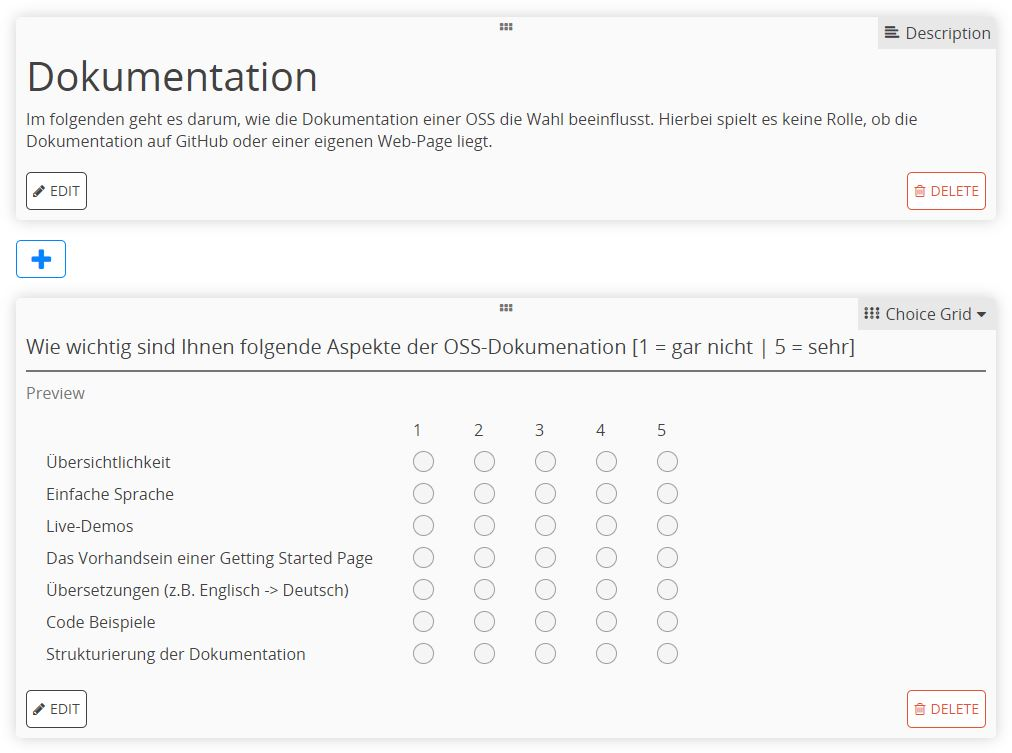
\includegraphics[scale=0.6]{figures/anhang/Frage_2.JPG}
\end{figure}


\subsubsection*{Wie wichtig sind Ihnen folgende Aspekte der OSS-Dokumentation [1=garnicht | 5 = sehr]}
\begin{table}[h]
    \begin{tabular}{l|c|c|c|c|c|}
                                                                     & \multicolumn{1}{l|}{\textbf{1}} & \multicolumn{1}{l|}{\textbf{2}} & \multicolumn{1}{l|}{\textbf{3}} & \multicolumn{1}{l|}{\textbf{4}} & \multicolumn{1}{l|}{\textbf{5}} \\ \hline
        \textbf{Übersichtlichkeit}                                   & 0                               & 6                               & 26                              & 124                             & 149                             \\ \hline
        \textbf{Einfache Sprache}                                    & 29                              & 59                              & 100                             & 87                              & 29                              \\ \hline
        \textbf{Live-Demos}                                          & 30                              & 89                              & 89                              & 66                              & 29                              \\ \hline
        \textbf{Das Vorhandensein einer Getting Started Page}        & 204                             & 54                              & 34                              & 6                               & 6                               \\ \hline
        \textbf{Übersetzungen (z.B. Englisch -\textgreater Deutsch)} & 5                               & 22                              & 56                              & 109                             & 109                             \\ \hline
        \textbf{Strukturierung der Dokumentation}                    & 3                               & 4                               & 28                              & 11                              & 157                             \\ \hline
    \end{tabular}%
\end{table}


\newpage
\subsubsection*{Die folgenden Punkte würden mich von der Nutzung eines OSS-Projekts abhalten oder mich möglicherweise dazu veranlassen, nach
    Alternativen zu suchen. [1 = Stimme ich garnicht zu | 5 = Stimme ich voll und ganz zu]}
\begin{table}[h]
    \begin{tabular}{l|c|c|c|c|c|}
                                               & \textbf{1} & \textbf{2} & \textbf{3} & \textbf{4} & \textbf{5} \\ \hline
        \textbf{Keine Code Beispiele}          & 5          & 26         & 45         & 91         & 137        \\ \hline
        \textbf{Schlechte Struktur}            & 2          & 25         & 68         & 110        & 100        \\ \hline
        \textbf{Komplexe Doku}                 & 12         & 55         & 109        & 85         & 43         \\ \hline
        \textbf{Fehlende Ubersetzung}          & 227        & 51         & 18         & 4          & 4          \\ \hline
        \textbf{Fehlende Getting Started Page} & 22         & 77         & 91         & 76         & 37         \\ \hline
    \end{tabular}%
\end{table}

\subsubsection*{Hat sie eine schlechte Dokumentation jemals dazu gebracht, ein alternatives Projekt zu wählen?}

249 haben für \textit{"Ja"} gestimmt, und 58 für \textit{"Nein"}.

% ------------------------------------------ Beliebtheit ----------------------------------------- %
\subsection{Beliebtheit}

Im folgenden Teil geht es um die Aspekte der Beliebtheit und wie diese Einfluss bei der Wahl eines Projektes haben.

\subsubsection*{Wie sehr achten Sie bei der Auswahl von OSS auf... [1 = garnicht | 5 = sehr]}

Die Frage bezüglich Trends bezeiht sich auf Trends wie sie auf z.B. StackOverflow, npm trends Google Trends oder ähnlichen
Plattformen zu finden sind.

\begin{table}[h]
    \begin{tabular}{l|c|c|c|c|c|}
                                                           & \textbf{1} & \textbf{2} & \textbf{3} & \textbf{4} & \textbf{5} \\ \hline
        \textbf{Anzahl der Downloads}                      & 33         & 49         & 67         & 118        & 40         \\ \hline
        \textbf{GitHub/GitLab Sterne}                      & 46         & 60         & 96         & 83         & 22         \\ \hline
        \textbf{Anzahl Contributor}                        & 54         & 82         & 100        & 51         & 20         \\ \hline
        \textbf{Trends}                                    & 105        & 84         & 69         & 40         & 9          \\ \hline
        \textbf{Anzahl Sponsoren}                          & 192        & 103        & 57         & 17         & 1          \\ \hline
        \textbf{Anzahl von StackOverflow Fragen/Antworten} & 89         & 50         & 83         & 64         & 21         \\ \hline
    \end{tabular}%
\end{table}


\subsubsection*{Hat die geringe Popularität eines Projekts Sie jemals davon abgehalten, es zu nutzen?}
140 haben für \textit{"Ja"} gestimmt, und 167 für \textit{"Nein"}.


% ------------------------------------------- Sponsoren ------------------------------------------ %
\subsection{Sponsoren}
Im folgenden geht es, um Sponsoren und dessen Einfluss bei der Wahl eines OSS-Projekts.
Da einige Open Source Projekte, wie Android von Google, von Unternehmen entwickelt werden sind diese nicht von
Sponsoren nicht abhängig und spielen für die folgenden Fragen daher keine Rolle.
Die Fragen beziehen sich daher auf Projekte, die von der Community entwickelt werden und auf
Sponsoren angewiesen sind. Beispielsweise VueJS oder PostgreSQL.

\subsubsection*{Bewerten Sie folgende Aussagen [1 = stimme NICHT zu | 5 = stimme voll und ganz zu]}

\begin{table}[h]
    \begin{tabular}{l|c|c|c|c|c|}
        \textbf{}                                   & \textbf{1} & \textbf{2} & \textbf{3} & \textbf{4} & \textbf{5} \\ \hline
        \textbf{Zukunftssicherer}                   & 26         & 34         & 11         & 110        & 26         \\ \hline
        \textbf{Projekt mit Sponsor wird bevorzugt} & 62         & 82         & 117        & 40         & 6          \\ \hline
        \textbf{Gesponsert ist besser}              & 45         & 69         & 135        & 47         & 11         \\ \hline
    \end{tabular}%
\end{table}

% ------------------------------------------ Devlopment ------------------------------------------ %
\newpage
\subsection{Devlopment}

Welchen Einfluss hat der Entwicklungsprozess bei der Auswahl eines Projektes.

\subsubsection*{Wie sehr achten Sie auf die Folgenden Punkte, wenn Sie ein Projekt wählen? [1 = gar nicht | 5 = sehr]}


\begin{table}[h]
    \begin{tabular}{l|c|c|c|c|c|}
                                                                & \textbf{1} & \textbf{2} & \textbf{3} & \textbf{4} & \textbf{5} \\ \hline
        \textbf{Anzahl der Maintainer}                          & 24         & 55         & 71         & 111        & 46         \\ \hline
        \textbf{Ticket/Issue Verhältnis Open/Closed}            & 44         & 62         & 97         & 89         & 15         \\ \hline
        \textbf{Regelmäßigkeit der Commits}                     & 24         & 47         & 95         & 102        & 39         \\ \hline
        \textbf{Aktualität des letzten commits}                 & 11         & 21         & 49         & 121        & 105        \\ \hline
        \textbf{Antwortzeit der Entwicklera auf Tickets/Issues} & 33         & 74         & 113        & 78         & 9          \\ \hline
    \end{tabular}%
\end{table}



\subsection*{Priorisierung der Kriterien}

In der letzten Frage sollten die Teilnehmer Kriterien sortieren nach Priorität sortieren. Die Aussage war:
\textit{Sortieren Sie nach den für Sie wichtigsten Kriterien bei der Auswahl von OSS.}
Das Tool hat je nach Platzierung die Kriterien bepunktet. Für Platz 1 gab es 5 Punkte, für Platz 2 gab es Platz 4 gab es 4 Punkte usw.

Folgende Auflistung hat sich entsprechend ergeben:

\begin{itemize}
    \item \textbf{[1329]} Punkte für Gute Dokumentation
    \item \textbf{[1165]} Punkte für Beliebtheit (Anzahl der Downloads, GitHub Stars etc.)
    \item \textbf{[794]} Punkte für Anzahl von offenen Issues/Tickets
    \item \textbf{[624]} Punkte für Trends (z.B. auf StackOverflow oder GoogleTrends etc)
    \item \textbf{[559]} Punkte für Projekt hat Sponsoren
\end{itemize}
